\section{SLAM}

There are not too many results to show in regards to the SLAM, as we do not get to test it on anything else than simulation until the car is ready, which is going to be some time after this project thesis is delivered. 

When simulating with false positives generated with a random Gaussian position, the frontend does not let any false positives through. This is of course not the best metric for performance, since detection systems don't really send false positives with completely random position. The ones they send are usually because of objects around the track, like walls, and will be spatially correlated. This means that the frontend will have to deal with false positives that cluster around particular areas. Detection data from last year shows that the false positives that get detected usually jump around a lot, so hopefully the frontend will spawn many new hypotheses that loose confidence, instead of associating to the same false positive and eventually sending it through to the backend. This is not possible to test at the moment unfortunately, since the data from last year isn't compatible with the current system. 

The time used for each iteration of the frontend when simulating one round of the \gls{FSG} Trackdrive 2018 is shown in figure \ref{Fig:FrontendTiming}. Similarly the time used for each iteration of the backend is shown in figure \ref{Fig:BackendTiming}. 

The \gls{RMS} error of the map that the \gls{SLAM} system has with ground truth after simulating the same track has been recorded over many runs with different amount of noise added to the detections. This error is plotted in figure \ref{Fig:SLAMERMS} as a function of the logarithm of the order of magnitude of the standard deviation of this noise.

\begin{figure}
    \centering
    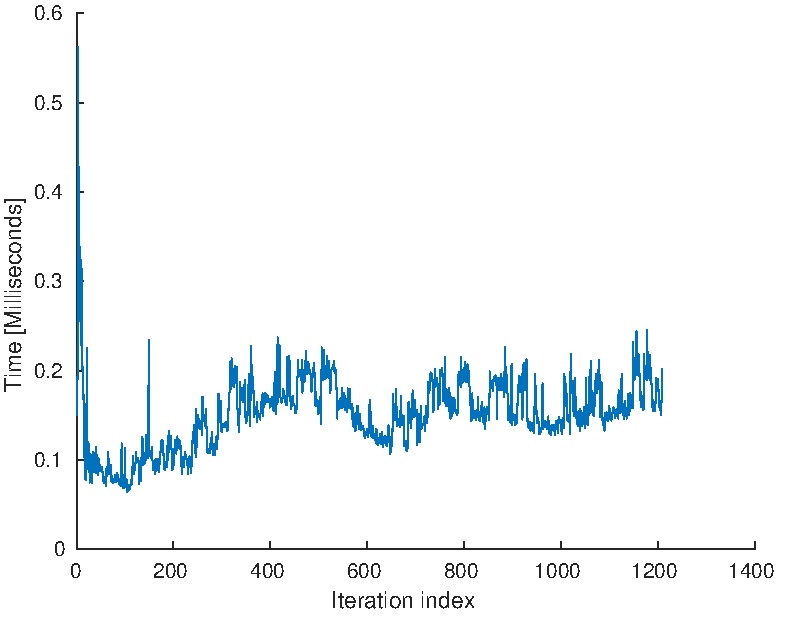
\includegraphics[width=0.8\linewidth]{0_Images/6_Results/FrontendTiming.pdf}
    \caption[Run time of the SLAM frontend.]
    {Run time of the SLAM frontend over time, when simulating with Gaussian noise on detection and odometry. The timing is from when the set of detection arrives from one of the detection systems to when it is done processing. Simulated using the track from FSG's Autocross event 2018.}
    \label{Fig:FrontendTiming}
\end{figure}

\begin{figure}
    \centering
    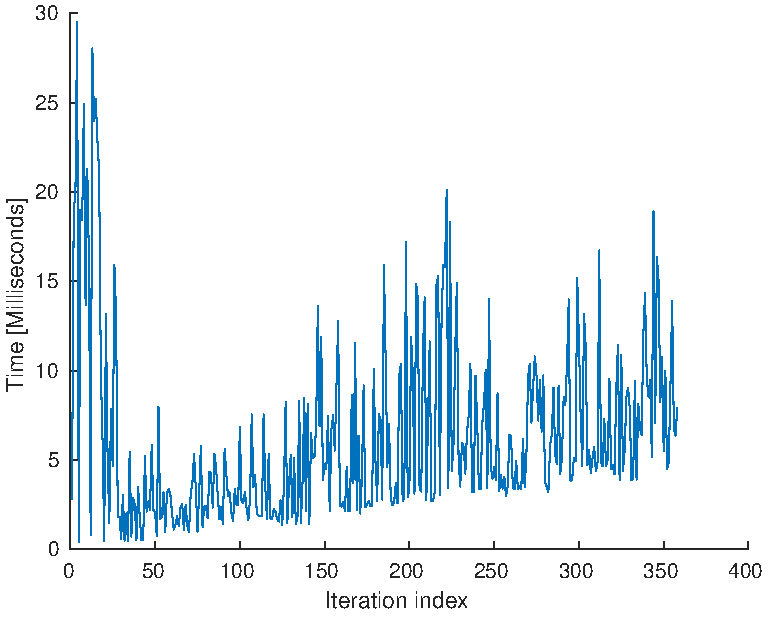
\includegraphics[width=0.8\linewidth]{0_Images/6_Results/BackendTiming.pdf}
    \caption[Run time of the SLAM backend.]
    {Run time of the SLAM backend over time, for one complete update. One update means adding all the new information to the graph, optimising the graph and then sending out the map and pose correction. Simulated using the track from FSG's Autocross event 2018.}
    \label{Fig:BackendTiming}
\end{figure}

\begin{figure}
    \centering
    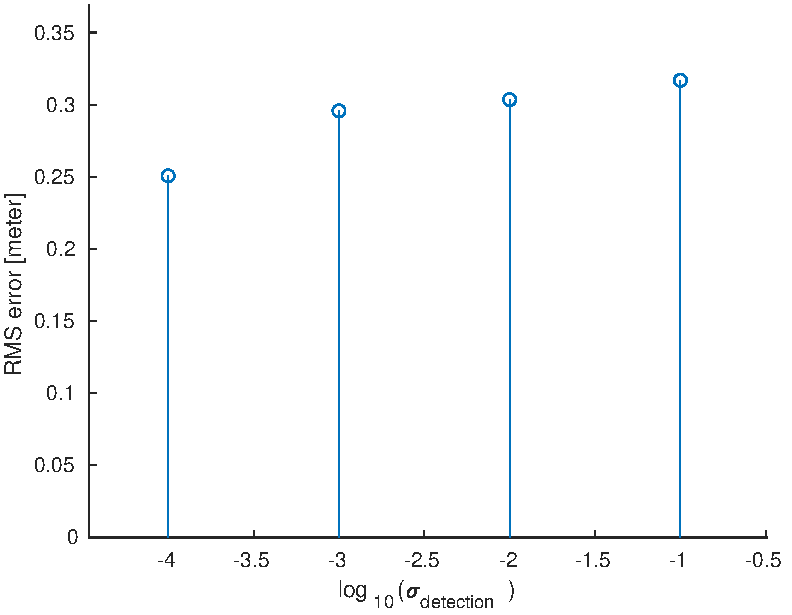
\includegraphics[width=0.8\linewidth]{0_Images/6_Results/SLAMERMS.pdf}
    \caption[SLAM RMS error.]
    {SLAM RMS error, as a function of the logarithm of standard deviation of the Gaussian noise added to the simulated detections. Simulated on one full round around the FSG autocross event 2018. Each RMS error value corresponds to the mean over ten simulations.}
    \label{Fig:SLAMERMS}
\end{figure}